\subsection*{Paikkajärjestelmät}

Merkitsemme lukuja yleensä \termi{kymmenjärjestelmä}{kymmenjärjestelmässä} eli \termi{lukujärjestelmä}{lukujärjestelmässä}, jossa on kymmenen \termi{numeromerkki}{numeromerkkiä}: $0, 1, 2, 3, 4, 5, 6, 7, 8, 9$. (Käyttämämme numeromerkit ovat nimeltään hindu-arabialaiset numerot.) Kymmenjärjestelmää kutsutaan myös \termi{desimaalijärjestelmä}{desimaalijärjestelmäksi}. Tunnetaan kulttuureja, joissa on käytetty pääasiallisesti jotakin muuta lukujärjestelmää.

Kymmenjärjestelmä on \termi{paikkajärjestelmä}{paikkajärjestelmä}, eli merkin paikka määrittää sen merkityksen.
Esimerkiksi luvussa $80$ merkin 8 merkitys on $8 \cdot 10^1$, mutta luvussa $820$ sen merkitys on $8 \cdot 10^2$.

Nykyään yleisimmät desimaalijärjestelmästä poikkeavat lukujärjestelmät ovat \termi{binäärijärjestelmä}{binääri}-, \termi{oktaalijärjestelmä}{oktaali}- ja \termi{heksadesimaalijärjestelmä}{heksadesimaalijärjestelmät}, joissa on 2, 8 ja 16 numeromerkkiä. Tietokoneet käsittelevät lukuja sisäisesti binäärijärjestelmässä, kun taas oktaali- ja heksadesimaalijärjestelmät ovat muutoin käteviä tietojenkäsittelytieteessä.

Binäärijärjestelmässä luvun muodostavia numeromerkkejä kutsutaan \termi{bitti}{biteiksi}. Bitti voi olla joko päällä (1) tai pois päältä (0), ja toteutus tietokoneessa vastaa esimerkiksi sitä, että johtimessa kulkee virta (1) tai ei (0).

%\begin{esimerkki}
%	$10,01_2 = 1 \cdot 2^1 + 0 \cdot 2^0 + 0 \cdot 2^{-1} + 1 \cdot 2^{-2} = 2,25_{10}$
%\end{esimerkki}

Kuusitoistajärjestelmässä tarvitaan numeroiden $0 \ldots \, 9$ lisäksi kuusi uutta numeromerkkiä. Tavaksi on vakiintunut käyttää kirjainmerkkejä $\mathrm{A, B, C, D, E, F}$. Ne vastaavat desimaalilukuja $10 \ldots \, 15$.

Useampaa järjestelmää käytettäessä, erityisesti muunnettaessa lukuja järjestelmästä toiseen, merkitään kantaluku luvun jälkeen alaindeksinä. Voimme esimerkiksi merkitä (desimaalijärjestelmän) lukua yhdeksäntoista $10011_{2}$, $23_{8}$, $19_{10}$ tai $13_{16}$.

Lukujärjestelmiä voidaan vaihtoehtoisesti merkitä kirjoittamalla niiden tunnus (Bin, Oct, Dec, Hex) luvun jälkeen.
Klassinen vitsi ''Miksi tietojenkäsittelytieteilijä sekoittaa halloweenin ja joulun? Koska 31 Oct = 25 Dec!'' perustuu siihen, että

\begin{align*}
	\text{halloween} \; = \; \text{31. lokakuuta} \; &= \; \text{31 Oct} \; = 31_8 = 3_{10} \cdot 8_{10} + 1_{10} \cdot 1_{10} \\
	= {25}_{10} &= \; \text{25 Dec} \; = \; \text{25. joulukuuta} \; = \; \text{joulupäivä.}
\end{align*}

\subsection*{Muut lukujärjestelmät}

Yleisesti tunnetaan myös joitakin lukujärjestelmiä, jotka eivät ole paikkajärjestelmiä.

\termi{tukkimiehen kirjanpito}{Tukkimiehen kirjanpidossa} toistetaan yhtä ainoaa merkkiä. Se on tavallaan 1-järjestelmä, mutta tällainen määrittely ei ole ongelmaton.

\begin{center}
	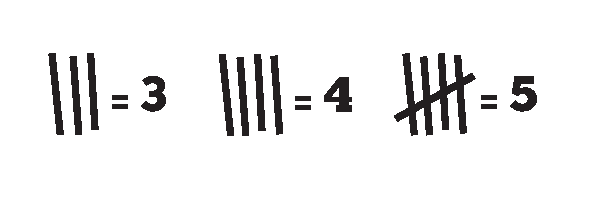
\includegraphics{pictures/Kuva1-1-tukkimiehenkirjanpito.pdf}
\end{center}

Hienostuneempi versio tukkimiehen kirjanpidosta ovat \termi{roomalaiset luvut}{roomalaiset luvut}, jotka nimensä mukaisesti olivat yleisin lukujärjestelmä antiikin Roomassa. Ne perustuvat havaintoon, että kun käytettävissä olevien merkkien määrää lisää, suuria lukuja voi kirjoittaa lyhyempään muotoon. Tilanne on verrattavissa vaikkapa kiinan kieleen, jossa on käytössä satoja erilaisia kirjoitusmerkkejä. Merkeissä on paljon muistettavaa, mutta toisaalta kokonaisen lauseen voi kirjoittaa vain parilla kirjoitusmerkillä.

Roomalaisia lukuja käytetään yhä nykyäänkin erityisesti järjestyksen merkitsemisessä.

Roomalaisten lukujen numeromerkit ovat I, V, X, L, C, D ja M. Ne vastaavat desimaalijärjestelmän lukuja seuraavalla tavalla:

\begin{equation*}
	\rm I=1\quad
	V=5\quad
	X=10\quad
	L=50\quad
	C=100\quad
	D=500\quad
	M=1\,000
\end{equation*}

Roomalaiset luvut merkitään kirjoittamalla merkkejä laskevassa järjestyksessä, poikkeuksena vähennyssääntö. Merkkien kokonaisarvo määrää luvun.

Vähennyssääntö tarkoittaa kuutta kaksimerkkistä ilmaisua:

\begin{equation*}
	\rm IV=4\quad
	IX=9\quad
	XL=40\quad
	XC=90\quad
	CD=400\quad
	CM=900
\end{equation*}

Luvussa voi olla vain kerran IV tai IX, vain kerran XL tai XC ja vain kerran CD tai CM.
Kaksimerkkisiin ilmaisuihin pätevät samat säännöt kuin numeromerkkeihinkin: I = $1$ ei voi edeltää numeroa IV = $4$, eikä IV = $4$ numeroa V = $5$. Lisäksi merkinnät IXV, XCL ja CMD eivät ole sallittuja. Oikea roomalainen luku minimoi käytettyjen merkkien määrän. Esimerkiksi VIV ei ole roomalainen luku, sillä IX on lyhyempi.

\termi{nolla}{Nollaa} roomalaisissa numeroissa ei ole; nolla nykyisessä merkityksessään kehitettiin Intiassa 800-luvulla jaa.

\begin{esimerkki}
	Roomalaisia lukuja:
	\alakohdat{
		§ III$=1+1+1=3$
		§ IX$=10-1=9$
		§ XII$=10+1+1=12$
		§ XIV$= 10 + (5 - 1) = 14$
		§ CDX$=500-100+10=410$
		§ MDC$=1\,000+500+100=1\,600$
	}
\end{esimerkki}

\begin{tehtavasivu}

\begin{tehtava}
Muunna seuraavat binääriluvut kymmenjärjestelmään.
	\alakohdat{
		§ $101,0_2$
		§ $1,00101_2$
		§ $100101,1101_2$
	}
\begin{vastaus}
	\alakohdat{
		§ $5,0_{10}$
		§ $1,15625_{10}$
		§ $37,8125_{10}$
	}
\end{vastaus}
\end{tehtava}

\begin{tehtava}
Muunna seuraavat luvut binäärijärjestelmään.
	\alakohdat{
		§ $7,0_{10}$
		§ $2,5_{10}$
		§ $11,1875_{10}$
	}
\begin{vastaus}
	\alakohdat{
		§ $111,0_2$
		§ $10,1_2$
		§ $1011,0011_2$
	}
\end{vastaus}
\end{tehtava}
%%Siirretty 1. kertauskokeesta tänne. Aleksi Sipola 15.12.2013
\begin{tehtava}
Muuta seuraavat kymmenjärjestelmän luvut heksadesimaaliluvuiksi. \\
	(a) $175$ \qquad
	(b) $384$.

\end{tehtava}

\begin{tehtava}
	Laske
	\alakohdat{
		§ $1101_2 \cdot 100_2$
		§ $1101001_2 \cdot 100000_2$
		§ $10110_2 \cdot 0,01_2$.
	}
	\begin{vastaus}
		\alakohdat{
			§ $110100_2$
			§ $110100100000_2$
			§ $101,1_2$
		}
	\end{vastaus}
\end{tehtava}

\begin{tehtava}
	$\star$ Mikä on suuruusjärjestyksessä 148. positiivinen kokonaisluku, jonka kymmenjärjestelmäesityksessä on vain nollia ja ykkösiä?
	\begin{vastaus}
		$10010100$
	\end{vastaus}
\end{tehtava}

\begin{tehtava}
Mitkä seuraavista ovat oikeita roomalaisia lukuja? Mitä ne ovat kymmenjärjestelmässä?
\alakohdat{
§ $CLI$
§ $IVX$
§ $VIZI$
§ $CCLI$
§ $CCCLXXXVI$
§ $CMVCI$
§ $MMDCXLIIII$
§ $CDXCIII$
§ $DCXLIX$
} 
\begin{vastaus}
\alakohdat{
§ $151$
§ Ei ole oikea roomalainen luku.
§ Ei ole oikea roomalainen luku.
§ $251$
§ $386$
§ Ei ole oikea roomalainen luku.
§ Ei ole oikea roomalainen luku.
§ $493$
§ $649$
}
\end{vastaus}
\end{tehtava}

\begin{tehtava}
Muuta seuraavat kymmenjärjestelmän luvut roomalaisiksi luvuiksi. Kuinka monta merkkiä tarvitaan luvun kirjoittamiseen?
\alakohdat{
§ $278$
§ $712$
§ $1478$
§ $3999$
}
\begin{vastaus}
\alakohdat{
§ $CCLXXVIII$, 9 merkkiä 
§ $DCCXII$, 6 merkkiä
§ $MCDLXXVIII$, 10 merkkiä
§ $MMMCMXCIX$, 9 merkkiä
}
\end{vastaus}
\end{tehtava}

\end{tehtavasivu}
